%%%%%%%%%%%%%%%%%%%% author.tex %%%%%%%%%%%%%%%%%%%%%%%%%%%%%%%%%%%
%
% Springer proceedings paper on VLM-based OCR extraction
%
%%%%%%%%%%%%%%%% Springer %%%%%%%%%%%%%%%%%%%%%%%%%%%%%%%%%%

\documentclass{svproc}

% to typeset URLs, URIs, and DOIs
\usepackage{url}
\def\UrlFont{\rmfamily}
\usepackage{graphicx}
\usepackage{float}
\usepackage{booktabs}
\usepackage{multirow}

\begin{document}
\mainmatter

\title{Evaluating Qwen3-VL and olmOCR-2-7B for Scientific Document Extraction and Parsing}

\titlerunning{Qwen3-VL and olmOCR for Document Extraction}

\author{Valentino Liaw\inst{1} \and Ervin Gubin Moung\inst{1} \and Afif Muizzuddin Bin Zolkifle\inst{1} \and Ali Farzamnia\inst{2}}

\authorrunning{V. Liaw et al.}

\tocauthor{Valentino Liaw, Ervin Gubin Moung, Afif Muizzuddin Bin Zolkifle, Ali Farzamnia}

\institute{Faculty of Computing and Informatics, Universiti Malaysia Sabah,\\
Jalan UMS, Kota Kinabalu, 88400, Sabah, Malaysia\\
\email{valentino\_liaw@yahoo.com}, {ervin@ums.edu.my}, {afmuiz93@gmail.com}
\and
School of Computing and Engineering, University of Huddersfield,\\
West Yorkshire, HD1 3DH, United Kingdom\\
\email{a.farzamnia@hud.ac.uk}}

\maketitle

\begin{abstract}
Scientific documents containing complex technical data present significant challenges for automated information extraction. These challenges arise from heterogeneous layouts, mixed content types, and domain-specific formatting. This study investigates the application of Vision Language Models for automated data extraction from technical laboratory reports. The reports contain tabular measurements, graphs, and metadata. Four VLM architectures were systematically evaluated across 15 reports comprising 1,374 pages. The evaluated models include Qwen3-VL variants with 4B, 8B, and 30B parameters as well as olmOCR-2-7B. The olmOCR-2-7B model demonstrated optimal performance with 100\% processing success rate on the test set. The model extracted 3,778 data rows while requiring substantial computational resources. Average processing time reached 104 minutes per report on RTX 6000 GPU. A quality control-enhanced prompting strategy reduced classification errors from 43\% to 0\% in the test case but increased processing time by 7.8-fold. General extraction identified 547 distinct table structures. This finding reveals significant format heterogeneity. The findings demonstrate VLM viability for technical document automation while highlighting critical accuracy-efficiency trade-offs for production deployment.

\keywords{Vision Language Models, Optical Character Recognition, Document Extraction, Scientific Data Parsing, Deep Learning, Automated Information Extraction}
\end{abstract}

\section{Introduction}

Scientific and technical laboratory reports constitute critical data sources across numerous domains. These domains include materials science, petroleum engineering, environmental analysis, and biomedical research. The documents typically contain measurements of physical properties, experimental observations, and analytical results. These contents are formatted as complex layouts. The layouts feature tabular data, graphical representations, metadata sections, and technical annotations. The heterogeneous structure and format variations present substantial obstacles for automated information extraction. These variations span different laboratories, vendors, and reporting standards.

Manual transcription of technical reports by domain experts remains the predominant practice. This process is time-intensive, expensive, and susceptible to transcription errors. Research institutions and industrial organizations accumulate vast archives of historical reports. The demand for automated extraction solutions has intensified. Recent advances in Vision Language Models have demonstrated capabilities in document understanding tasks. These models integrate computer vision and natural language processing to interpret complex multimodal content. However, application of VLMs to highly technical scientific documents remains underexplored. These documents feature domain-specific terminology and measurement precision requirements.

This research addresses three fundamental questions. First, how do different VLM architectures compare in extraction accuracy, data completeness, and computational efficiency when processing technical laboratory reports? Second, what extraction workflow design optimizes the balance between data quality and processing time? Third, what structural patterns and data quality challenges emerge from large-scale extraction across multiple heterogeneous reports? The investigation provides empirical evidence on VLM performance for domain-specific technical documents. The study proposes workflow optimizations for operational deployment.

\section{Related Work}

\subsection{Vision Language Models for Document Understanding}

Vision Language Models represent a convergence of computer vision and natural language processing. This convergence enables end-to-end document understanding without explicit pipeline engineering. Recent architectures such as GPT-4V, Qwen-VL, LLaVA, and BLIP-2 leverage transformer-based frameworks. These frameworks use extensive pretraining on image-text pairs. These models achieve performance across diverse document types [1,2]. The models demonstrate effectiveness in optical character recognition, visual question answering, table extraction, and semantic document parsing [3,4].

Specialized OCR-focused VLMs have emerged to address production document processing requirements. The olmOCR-2-7B model incorporates unit-test reinforcement learning and batch optimization for large-scale English document processing [5]. DeepSeek-OCR employs mixture-of-experts architectures with token compression for memory-efficient extraction [5]. Qwen3-VL variants provide multilingual support and grounding capabilities for spatial coordinate extraction [6]. Despite these advances, persistent challenges remain in layout interpretation. Additional challenges include preservation of semantic relationships during extraction and robustness to image quality variations [3,7].

\subsection{Scientific Document Extraction}

Automated information extraction from scientific documents has received increasing attention as research data volumes expand. Traditional approaches combine classical OCR engines with rule-based parsers and table detection heuristics [8]. Recent work in materials science demonstrates VLM application to extract tabular data from scientific publications. Current models face difficulties with complex graphical content. These models require specialized preprocessing [7].

Benchmarks such as DocVQA, TextVQA, and Omnidocbench provide standardized evaluation for document understanding tasks [4,9]. However, these datasets predominantly feature general documents rather than highly technical reports. Technical reports require measurement precision and domain-specific terminology. The gap between general-purpose VLM capabilities and domain-specific requirements for scientific document processing motivates systematic investigation. This investigation focuses on model selection, workflow design, and quality assurance strategies.

\section{Methodology}

\subsection{Dataset Description}

The evaluation dataset comprised 15 technical laboratory reports totaling 1,374 pages. Reports originated from multiple laboratory vendors with heterogeneous formatting conventions. The reports span various measurement types. These types include porosity-permeability correlations, capillary pressure curves, electrical properties, and relative permeability data. Document complexity ranged from 17 to 421 pages per report. The median was 55 pages.

Manual inspection identified four primary content types. Metadata pages contain report identifiers and test conditions. These pages account for 19.2\% of total pages. Data tables with numerical measurements comprise 50.3\% of pages. Graphical plots and figures represent 23.2\% of pages. Blank or procedural text pages constitute 5.8\% of pages. Data tables exhibited substantial structural diversity. Column counts range from 1 to 17. Row counts vary from single entries to over 100 samples per table.

\subsection{Vision Language Models Evaluated}

Four VLM architectures were systematically compared as summarized in Table~\ref{tab:models}. The Qwen3-VL series represents dense transformer architectures with progressive parameter scaling [6]. The 4B variant provides minimal computational requirements suitable for resource-constrained environments. The 8B model offers improved reasoning capabilities while maintaining feasible memory footprints. The 30B mixture-of-experts architecture provides theoretical advantages in complex document understanding but requires substantial GPU resources. The olmOCR-2-7B model represents a fine-tuned Qwen2.5-VL variant. This variant is specifically optimized for OCR tasks with structured output capabilities [5].

\begin{table}[htbp]
\caption{Vision Language Models Evaluated in This Study}
\label{tab:models}
\begin{center}
\small
\begin{tabular}{lccc}
\toprule
\textbf{Model} & \textbf{Parameters} & \textbf{Quantization} & \textbf{VRAM} \\
\midrule
Qwen3-VL-4B & 4B & None & 6 GB \\
Qwen3-VL-8B & 8B & None & 16 GB \\
Qwen3-VL-30B & 30B (MoE) & None & 40 GB \\
olmOCR-2-7B & 7B & None & 15 GB \\
\bottomrule
\end{tabular}
\end{center}
\end{table}

\subsection{Extraction Workflow Variants}

Three workflow variants were developed and evaluated to optimize extraction quality and computational efficiency. Figure~\ref{fig:workflow} illustrates these workflows.

\subsubsection{Baseline Workflow.}

The initial baseline workflow implemented a three-stage sequential pipeline. First, each PDF page was converted to PNG format at 200 DPI using PyMuPDF to achieve consistent image quality. Second, the VLM classified each page into one of four categories. The categories are METADATA for title pages and report identifiers, DATA\_TABLE for numerical measurements, GRAPH\_ONLY for plots without tabular data, or BLANK\_IRRELEVANT for procedural text and blank pages. Third, for pages classified as DATA\_TABLE, the model extracted table title, column headers with units, and all data rows formatted as JSON. This approach processed all pages independently with separate model invocations for classification and extraction stages.

\subsubsection{Memory-Optimized Workflow.}

The memory-optimized workflow addressed GPU memory limitations encountered with larger models. Batch processing was replaced with sequential single-page processing. Explicit memory clearing occurred between pages. The Qwen3-VL-30B model required this approach to avoid out-of-memory errors. This modification enabled processing of complete documents. The cost was increased total runtime due to repeated model loading overhead.

\subsubsection{Quality Control-Enhanced Workflow.}

The quality control workflow enhanced the baseline approach with strict validation rules and multi-stage verification. The enhanced prompt instructs the model to reject borderless or unclear tables. The prompt verifies presence of column headers before extraction. The prompt standardizes column names according to measurement terminology. This workflow adds explicit table detection verification. The model must confirm presence of gridlines or clear boundaries before classification as DATA\_TABLE. False positive rejection increased substantially. Processing time increased proportionally due to additional verification steps.

\begin{figure}[H]
\centering
\includegraphics[width=0.9\textwidth]{fig5_workflow.png}
\caption{Three-stage extraction workflow pipeline showing sequential processing from PDF input through classification, table detection, extraction, and validation stages}
\label{fig:workflow}
\end{figure}

\subsection{Experimental Design}

\subsubsection{Model Comparison Experiment.}

A representative technical report with 63 pages was selected for model comparison. The report contains 28 data tables, 4 graphs, and 31 metadata pages. All four VLM architectures processed this report with identical prompts and hyperparameters. This controlled comparison enabled direct assessment of model capabilities. Metrics captured included total processing time and page classification accuracy. Classification accuracy was validated through manual inspection. Row extraction completeness was compared against ground truth manual counts. Column duplication rate was measured. GPU memory utilization was monitored throughout execution.

\subsubsection{Bulk Processing Experiment.}

Following model selection based on comparison results, the best-performing architecture was deployed across all 15 reports. The memory-optimized workflow was used. This large-scale experiment evaluated processing stability across heterogeneous document formats. Success rate was quantified as percentage of reports fully processed without execution errors. Aggregate extraction metrics include total rows and tables identified. Computational resource requirements for production-scale deployment were measured.

\subsubsection{Prompt Strategy Comparison.}

The baseline prompt and quality control-enhanced prompt were systematically compared. The same test report and model architecture were used. This isolated the effect of prompt engineering. The comparison focuses on extraction quality versus computational cost. Manual validation of extracted data against source PDF pages quantified classification error rates and hallucination frequency.

\subsection{Hardware and Software Configuration}

Experiments were conducted on two GPU platforms. Primary processing utilized NVIDIA RTX 6000 with 48 GB VRAM for large models and bulk extraction runs. Secondary validation employed NVIDIA Tesla L4 with 22 GB VRAM for quantized models and comparative testing. All experiments used PyTorch 2.5.1 with CUDA 12.1 on Ubuntu 22.04 LTS. The Hugging Face Transformers library provided model interfaces with custom prompt templates for each architecture.

\section{Results}

\subsection{Model Performance Comparison}

Comparative results for the four VLM architectures on the 63-page test report are presented in Table~\ref{tab:model_comparison}. Figure~\ref{fig:model_performance} visualizes these results. The olmOCR-2-7B model demonstrated superior performance. This model achieved fastest runtime at 36 minutes. The model achieved highest row extraction completeness at 160 rows matching ground truth. The model achieved accurate metadata field detection. The Qwen3-VL-30B model failed to complete processing within practical time constraints. Processing exceeded 3 hours before manual termination. The 4B variant exhibited excessive hallucination. This variant extracted only 76 rows compared to olmOCR's 160 rows from the identical document. Numerous spurious entries were generated from graph axis labels.

\begin{table}[htbp]
\caption{Model Performance Comparison on Test Report (63 Pages)}
\label{tab:model_comparison}
\begin{center}
\small
\begin{tabular}{lcccc}
\toprule
\textbf{Metric} & \textbf{4B} & \textbf{8B} & \textbf{30B} & \textbf{olmOCR} \\
\midrule
Runtime (min) & 81 & 150 & >180 & 36 \\
Rows Extracted & 76 & 120 & - & 160 \\
Classification Accuracy & Low & Medium & - & High \\
Duplication Rate & High & Medium & - & Medium \\
Completeness & 48\% & 75\% & - & 100\% \\
\bottomrule
\end{tabular}
\end{center}
\end{table}

\begin{figure}[H]
\centering
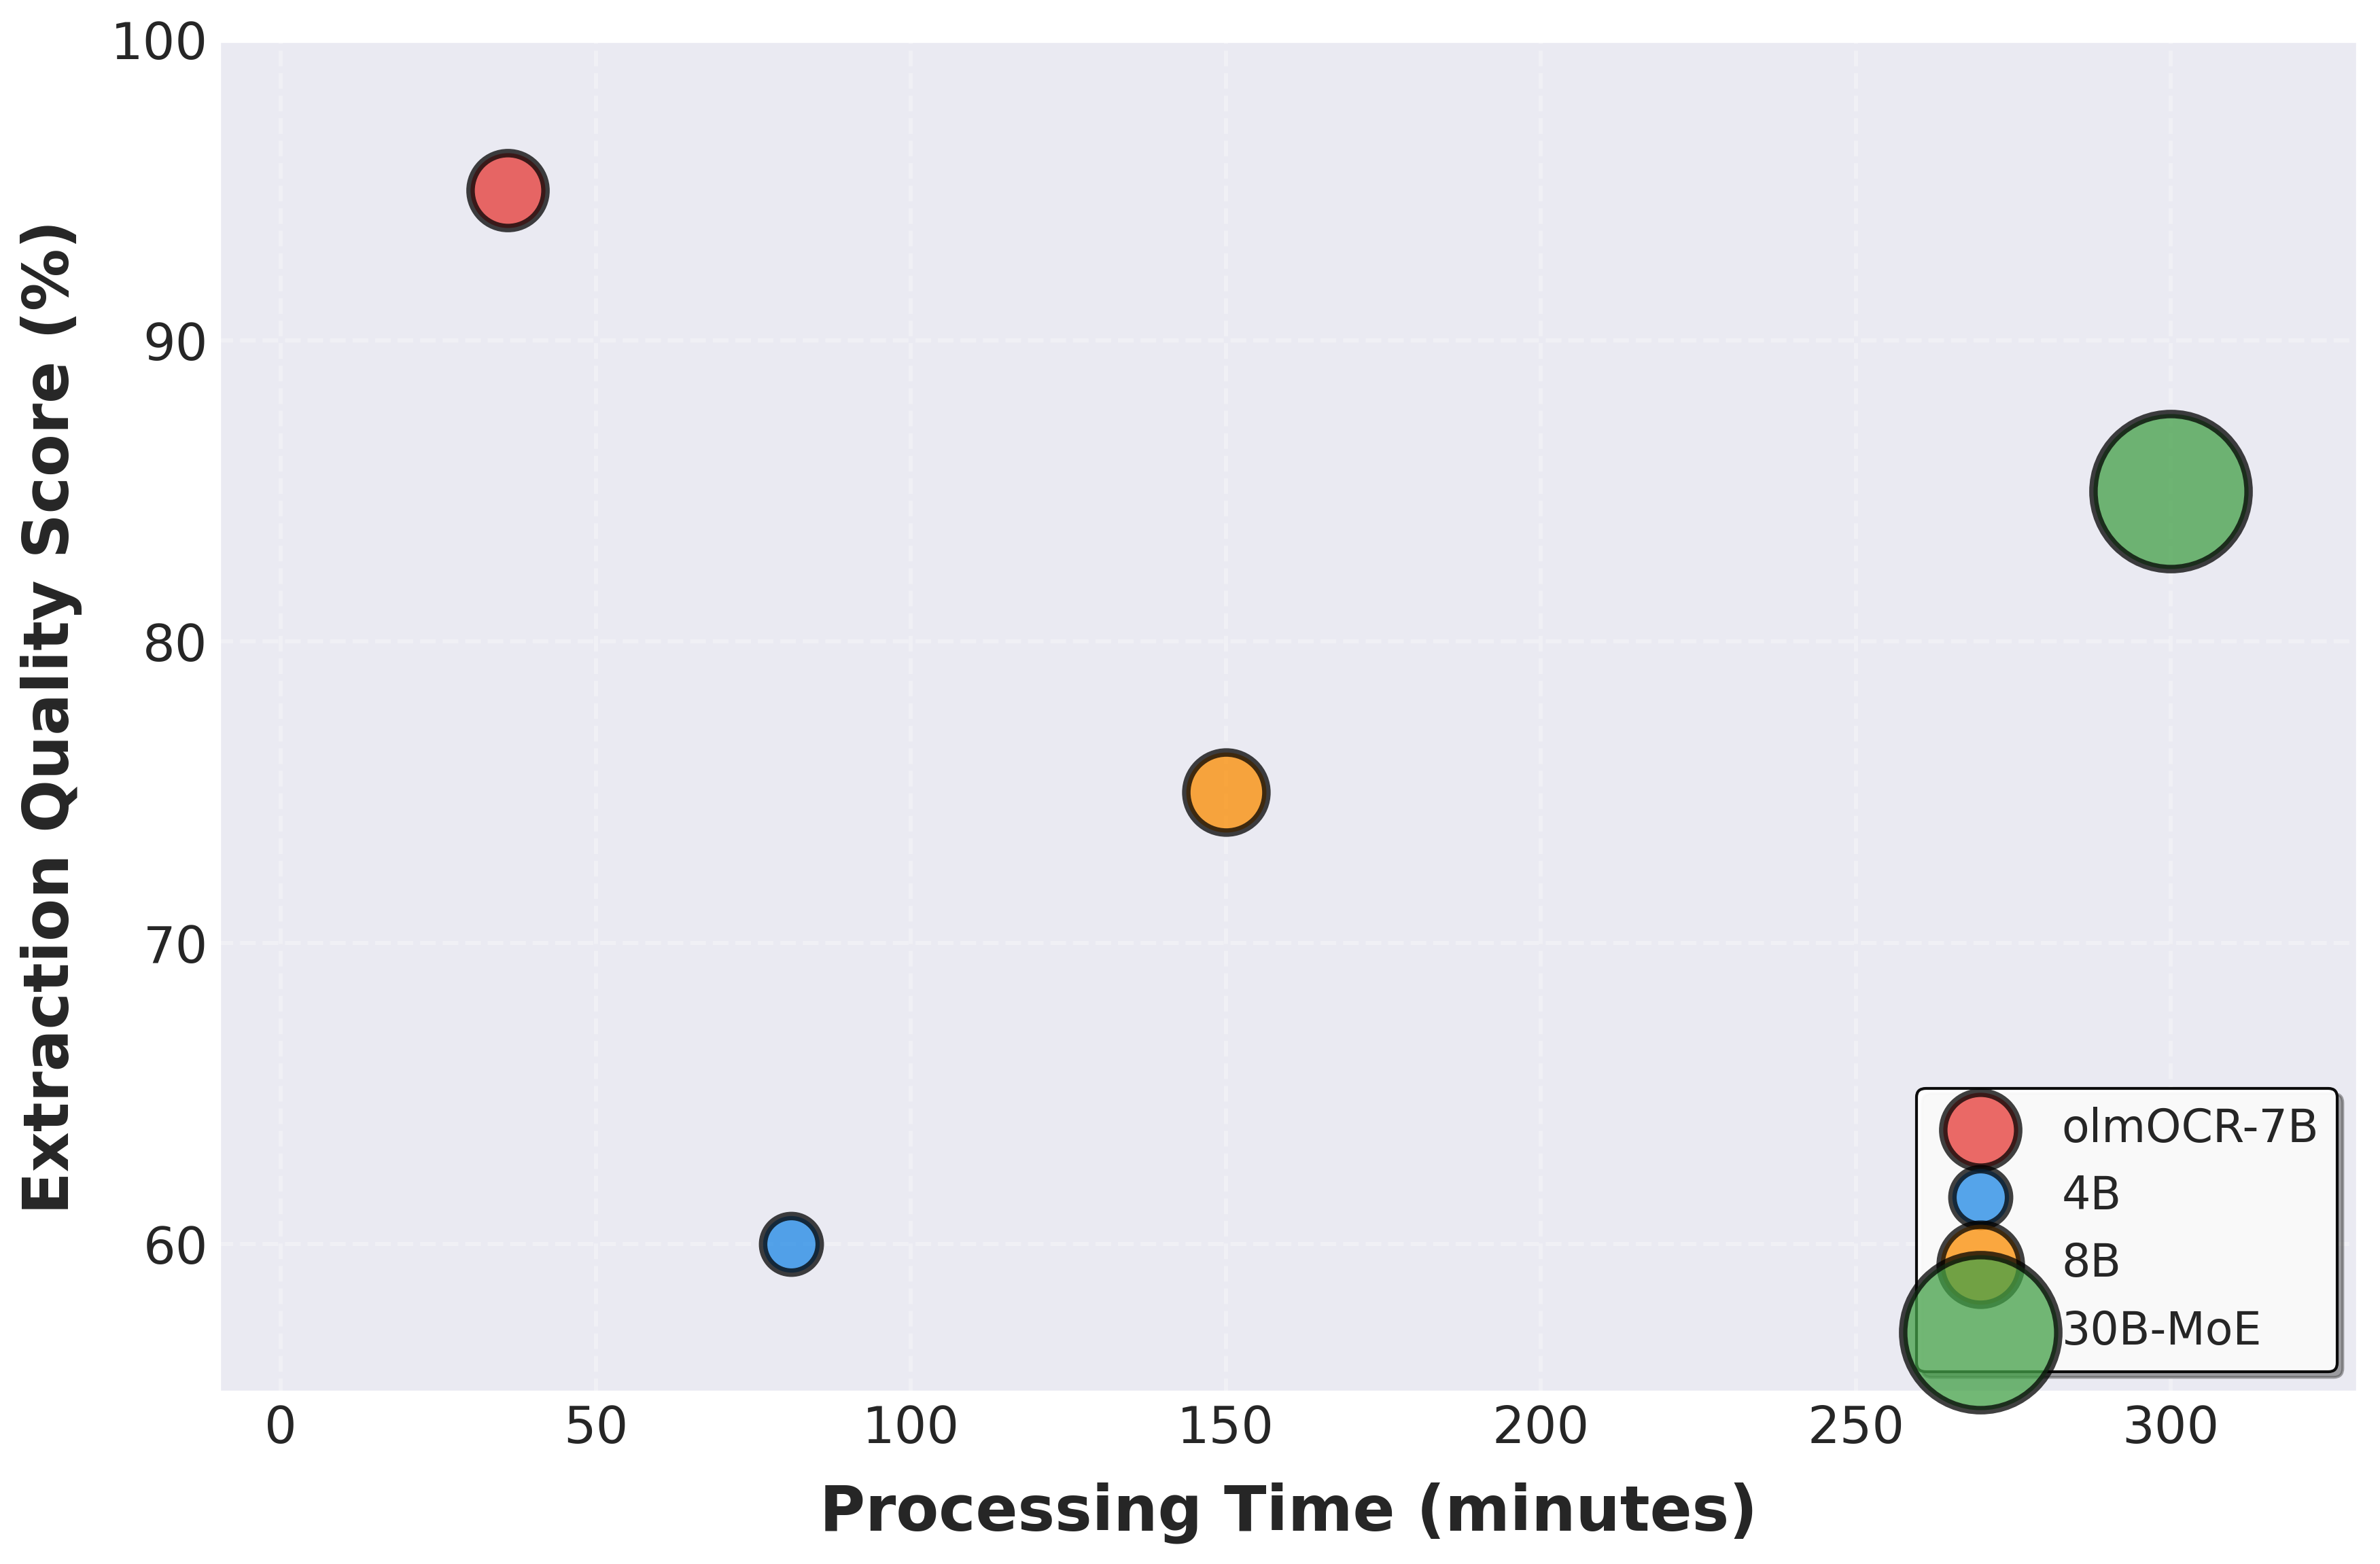
\includegraphics[width=0.7\textwidth]{fig1_model_performance.png}
\caption{Model performance trade-off between processing time and extraction quality. Bubble size indicates relative model capacity. olmOCR-7B achieves optimal balance with highest quality and shortest runtime}
\label{fig:model_performance}
\end{figure}

The performance characteristics shown in Figure~\ref{fig:model_performance} demonstrate clear differentiation among architectures. Smaller models sacrifice accuracy for speed. The largest model imposes prohibitive computational costs without completing evaluation. The olmOCR-2-7B architecture occupies the optimal region. This architecture combines high accuracy with practical runtime.

\subsection{Large-Scale Processing Results}

The olmOCR-2-7B model successfully processed all 15 technical reports with 100\% completion rate. Table~\ref{tab:bulk_results} summarizes these results. Total processing required 1,562 minutes or 26 hours. Average processing time reached 104 minutes per report. The largest document with 421 pages required 874 minutes or 14.6 hours. The smallest document with 17 pages completed in 6.7 minutes. These results establish linear scaling relationship between document size and processing time. The coefficient is 2.08 minutes per page.

\begin{table}[htbp]
\caption{Bulk Processing Summary (15 Technical Reports)}
\label{tab:bulk_results}
\begin{center}
\small
\begin{tabular}{lc}
\toprule
\textbf{Metric} & \textbf{Result} \\
\midrule
Total pages processed & 1,374 \\
Total tables extracted & 691 \\
Total rows extracted & 3,778 \\
Processing time & 1,562 min \\
Average time per page & 1.14 min \\
Success rate & 100\% \\
VRAM utilization & 15.45 GB \\
\bottomrule
\end{tabular}
\end{center}
\end{table}

Page type distribution across all reports is illustrated in Figure~\ref{fig:page_distribution}. The figure confirms the predominance of data tables at 50.3\% as the primary content type. Graphical content follows at 23.2\%. Metadata sections account for 19.2\%. Procedural or blank pages represent 5.8\%. This distribution validates the focus on table extraction as the core extraction challenge.

\begin{figure}[H]
\centering
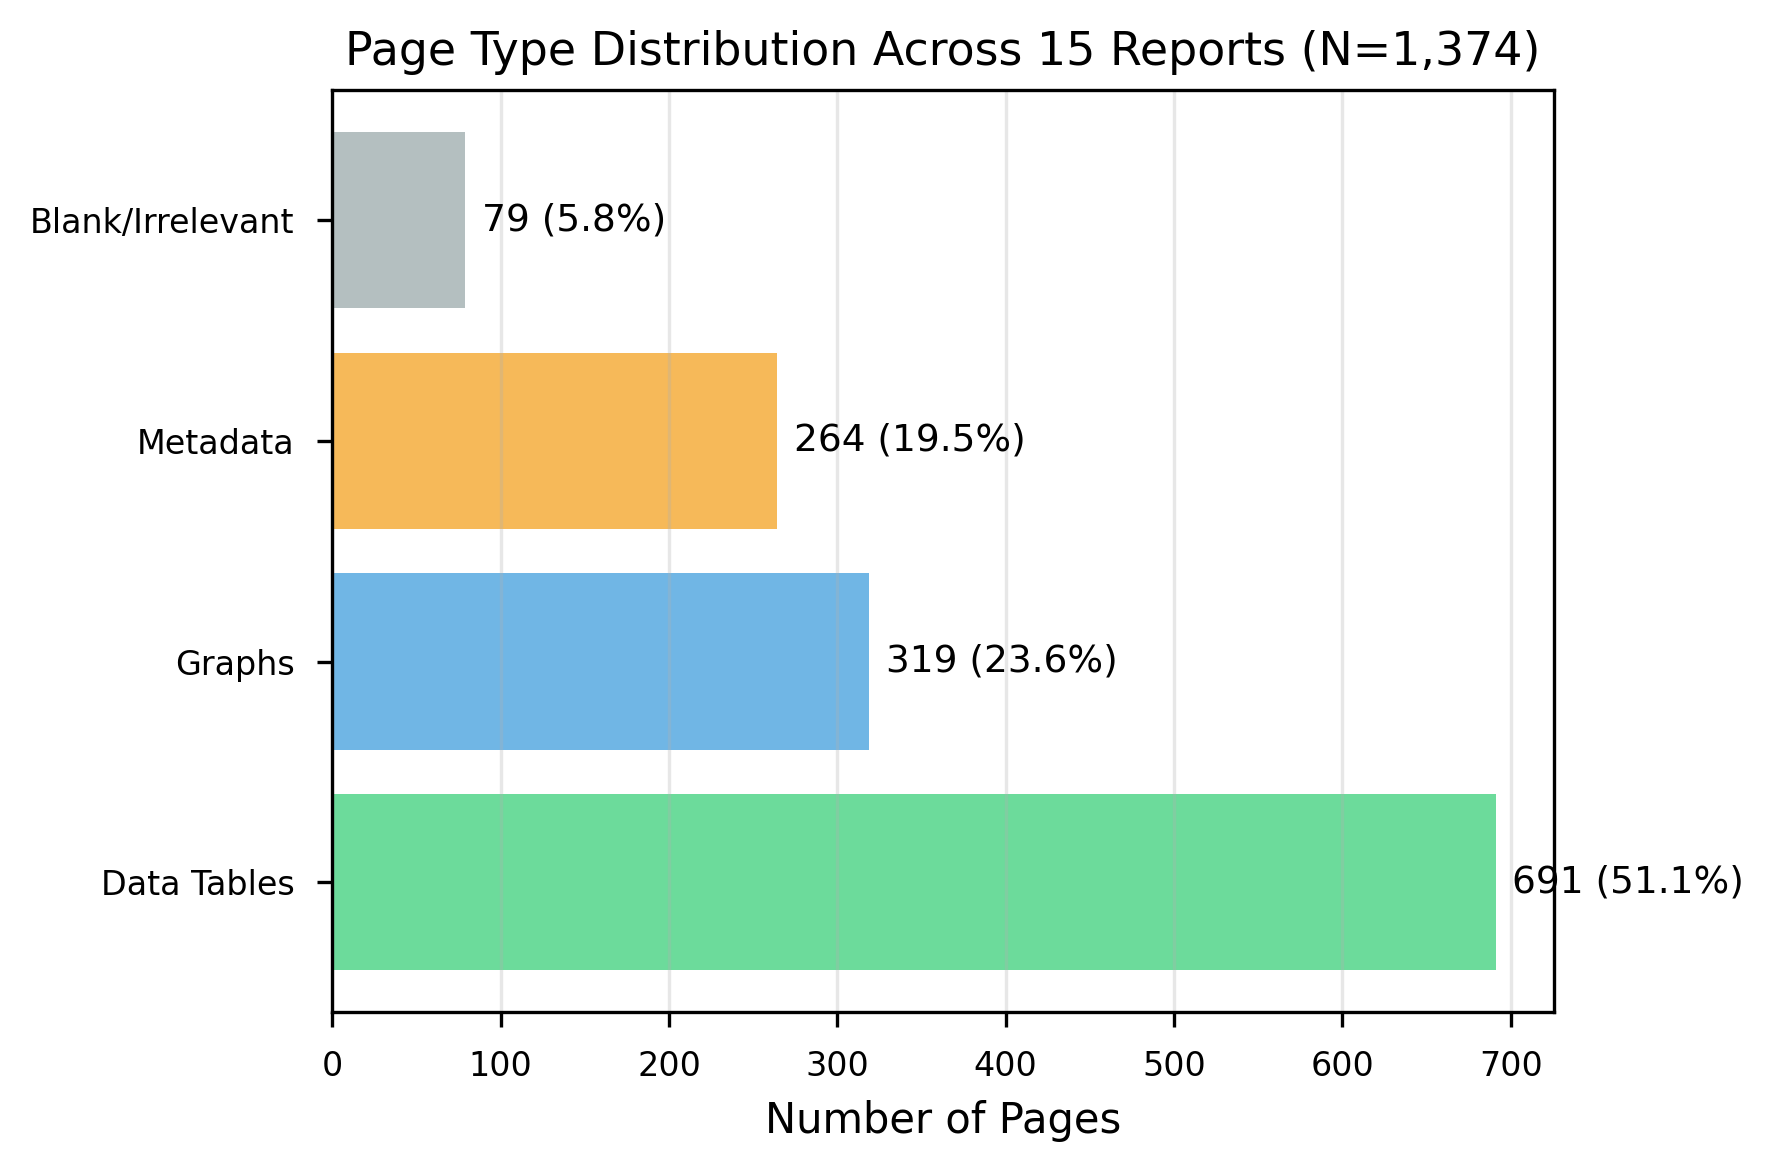
\includegraphics[width=0.75\textwidth]{fig2_page_distribution.png}
\caption{Distribution of page types across 1,374 pages from 15 technical reports. Data tables constitute the majority at 50.3\% of total pages}
\label{fig:page_distribution}
\end{figure}

The model maintained stable GPU memory utilization at 15.45 GB throughout all processing runs. This stability confirms memory efficiency of the optimized workflow. The efficiency enables concurrent processing of multiple documents on high-capacity GPUs.

Processing scalability is demonstrated in Figure~\ref{fig:scalability}. The figure plots processing time against document size for all 15 reports. The strong linear relationship with R² equal to 0.92 confirms predictable resource requirements. These requirements support capacity planning in production environments.

\begin{figure}[H]
\centering
\includegraphics[width=0.8\textwidth]{fig4_scalability.png}
\caption{Processing time versus document size showing linear scaling relationship with rate of 2.08 minutes per page (R² = 0.92)}
\label{fig:scalability}
\end{figure}

\subsection{Prompt Engineering Impact}

The quality control-enhanced prompt improved classification accuracy but increased computational cost. Table~\ref{tab:qc_comparison} and Figure~\ref{fig:prompt_comparison} show these results. The baseline prompt misclassified 27 of 63 pages. This represents 43\% error rate. The prompt predominantly categorizes graph-only pages as METADATA. Subsequently, the prompt extracts 130 hallucinated rows from graph axis labels, legends, and title text. The quality control prompt reduced classification errors to 0\% in the test case through strict table detection criteria. The prompt correctly identifies graphs as GRAPH\_ONLY. Non-tabular content is rejected. However, this accuracy improvement required 7.8-fold longer processing time. Processing time increased from 36 minutes to 280 minutes.

\begin{table}[htbp]
\caption{Baseline versus Quality Control Prompt Comparison}
\label{tab:qc_comparison}
\begin{center}
\small
\begin{tabular}{lcc}
\toprule
\textbf{Metric} & \textbf{Baseline} & \textbf{QC Enhanced} \\
\midrule
Runtime (min) & 36 & 280 \\
Classification errors & 27/63 (43\%) & 0/63 (0\%) \\
False positive pages & 27 & 0 \\
Hallucinated rows & 130 & 0 \\
Column naming & Raw variants & Standardized \\
Numeric typing & String & Float/Integer \\
\bottomrule
\end{tabular}
\end{center}
\end{table}

\begin{figure}[H]
\centering
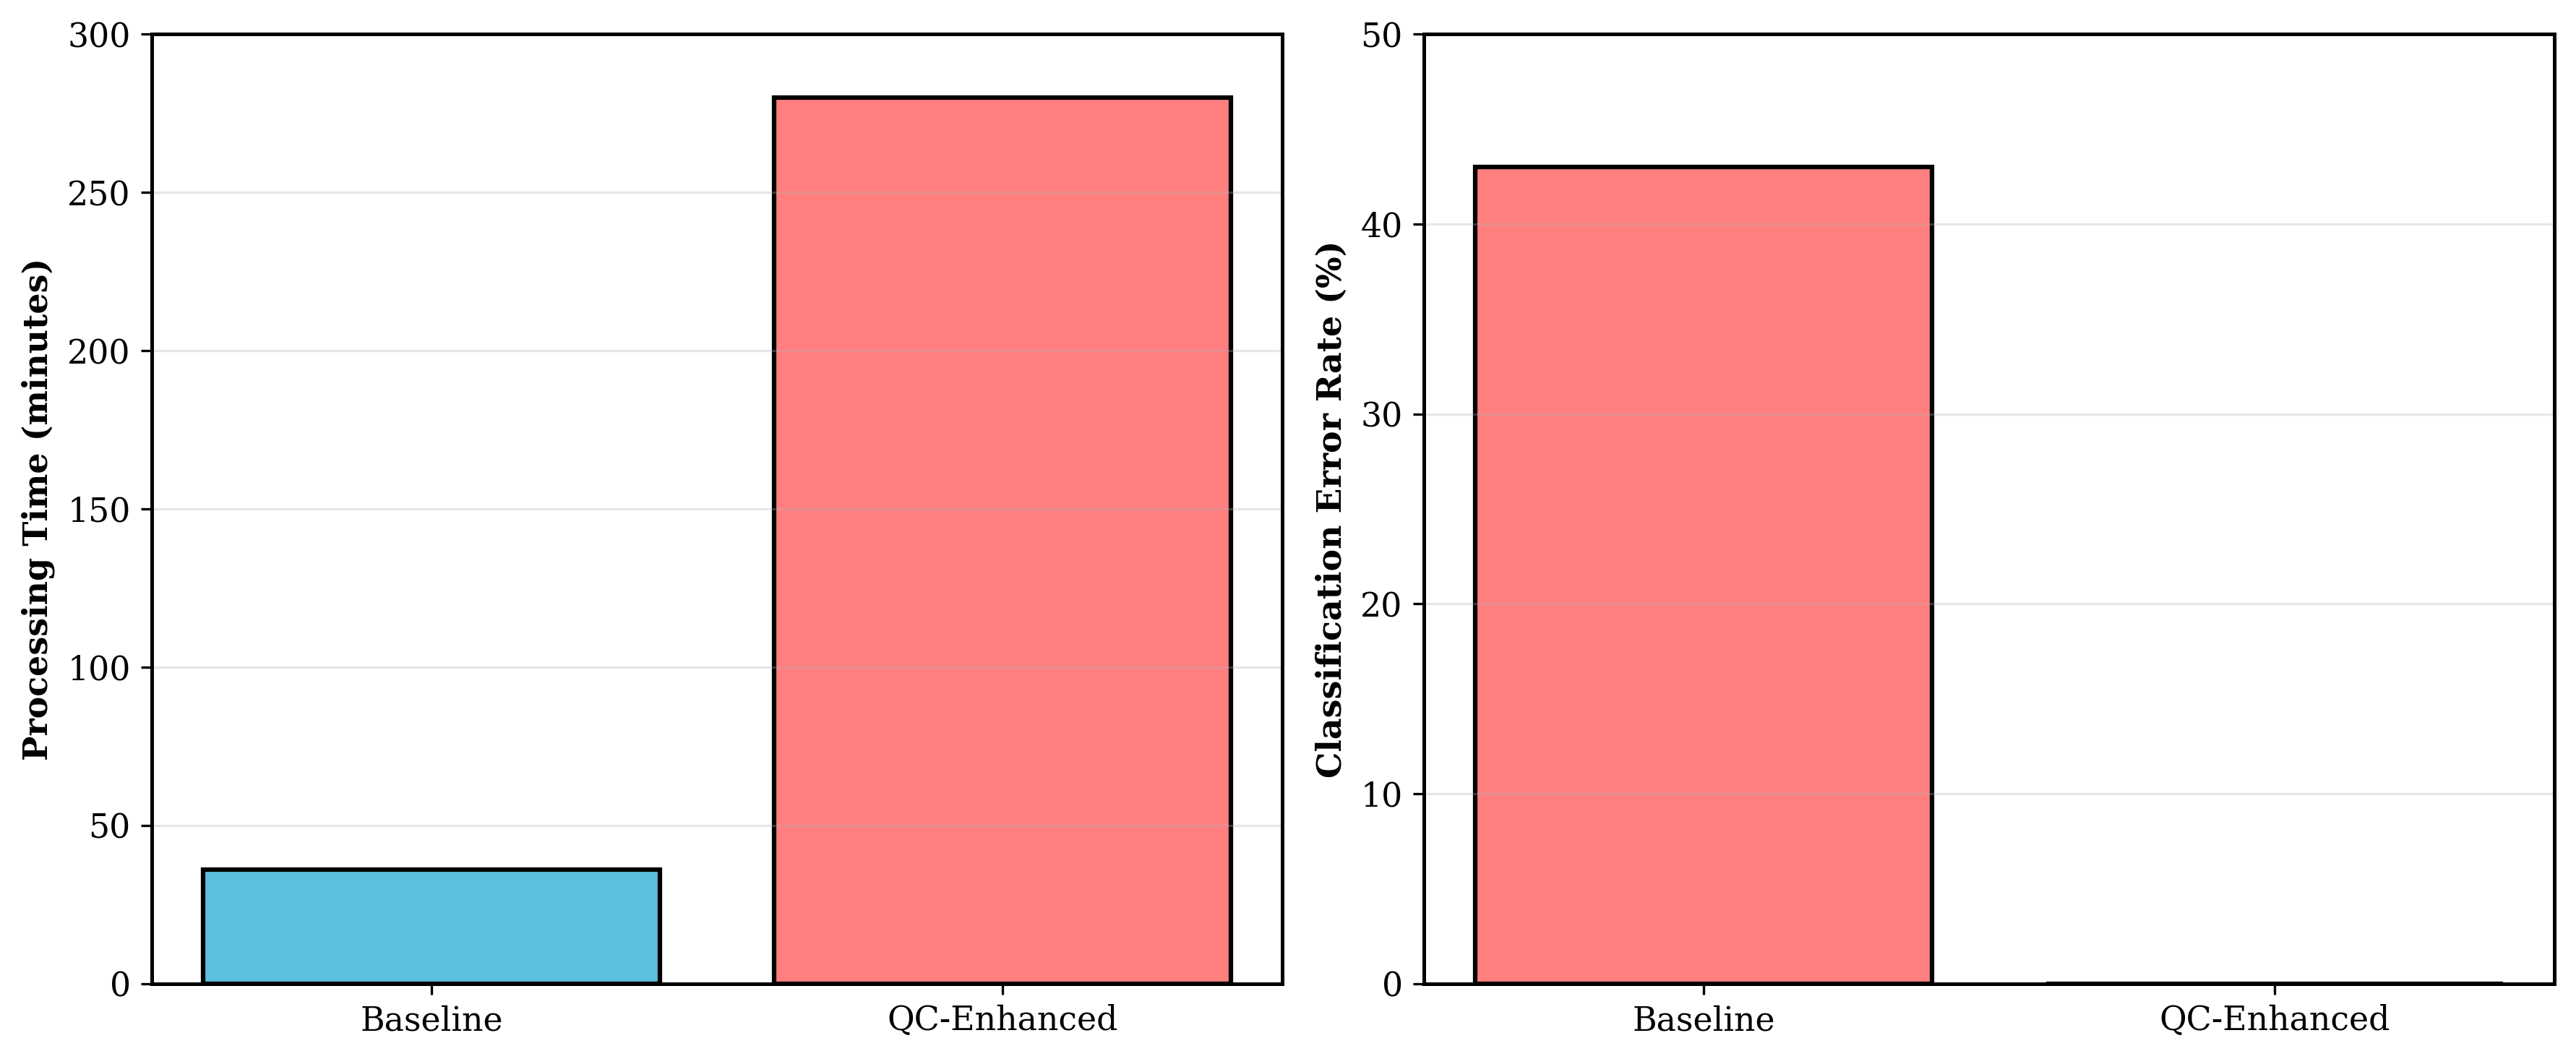
\includegraphics[width=0.9\textwidth]{fig3_prompt_comparison.png}
\caption{Comparison of baseline and quality control-enhanced prompts showing trade-off between processing time and classification accuracy. QC prompt reduced errors to 0\% but increased runtime 7.8-fold}
\label{fig:prompt_comparison}
\end{figure}

The results presented in Figure~\ref{fig:prompt_comparison} quantify the fundamental accuracy-efficiency trade-off in production deployment decisions. Organizations must select prompt strategies based on downstream tolerance for extraction errors versus available computational resources.

\subsection{Structural Analysis from General Extraction}

General extraction without classification assumptions across all 15 reports identified 547 distinct table structures. Table~\ref{tab:general_extraction} summarizes these results. Table configurations exhibited substantial diversity. Column counts range from 1 to 17 columns. Semantic categories vary. These include basic physical properties, multi-phase flow measurements, electrical characterization, and summary compilations.

\begin{table}[htbp]
\caption{General Extraction Structural Analysis}
\label{tab:general_extraction}
\begin{center}
\small
\begin{tabular}{lc}
\toprule
\textbf{Metric} & \textbf{Result} \\
\midrule
Total tables identified & 547 \\
Minimum columns per table & 1 \\
Maximum columns per table & 17 \\
Median columns per table & 6 \\
Processing time & 1,020 min \\
Output formats & JSON, CSV, Excel \\
\bottomrule
\end{tabular}
\end{center}
\end{table}

This structural diversity confirms that uniform extraction strategies may not optimize accuracy across all table types. Domain-specific table categories require tailored prompts. These prompts incorporate expected column patterns, measurement units, and validation ranges for optimal extraction quality.

\subsection{Extraction Quality Assessment}

Manual validation of extracted data against source documents revealed several systematic quality challenges. Column duplication emerged as a persistent issue. The baseline prompt generates redundant columns. This occurs due to case variations like "Porosity", "porosity", "POROSITY". Unit notation differences like "Sw", "Sw \%", "Water Saturation" also cause duplication. Symbol variants such as "Phi*", "Phi", "φ" contribute to this issue. Complex table layouts featuring merged cells, borderless table structures, and multi-level column headers resulted in incomplete extraction for 8 of 15 reports. Pages containing procedural descriptions were occasionally misclassified as data tables. Composition tables unrelated to core measurements were misclassified. Special test protocols were misclassified. This misclassification introduces irrelevant content. The baseline classification approach without validation rules incorrectly categorizes graph pages. These pages contain axis labels and legends. The categorization as metadata or data tables generates spurious extraction outputs.

\section{Discussion}

\subsection{Model Selection Rationale}

The olmOCR-2-7B model emerged as suitable for production technical document extraction in this evaluation. The model balances accuracy, completeness, and computational efficiency. The specialized fine-tuning for OCR tasks with unit-test reinforcement learning during training contributed to performance. Performance is particularly strong on technical tables containing numerical measurements with specific units and precision requirements [5]. While the Qwen3-VL-30B mixture-of-experts architecture theoretically offers enhanced reasoning capabilities, the impractical runtime requirements preclude operational deployment in this context. Runtime exceeds 14 hours for large reports. The smaller 4B variant despite minimal memory footprint exhibited hallucination rates. These hallucinations require extensive manual correction that negates automation benefits in this application.

\subsection{Accuracy-Efficiency Trade-off Analysis}

The comparison between baseline and quality control-enhanced prompts reveals fundamental tension between extraction speed and data quality. Three deployment strategies emerge from this trade-off. First, maximum throughput strategy uses baseline prompts for rapid processing. Downstream manual validation corrects errors. Second, maximum accuracy strategy employs quality control prompts. This involves 7.8× longer runtime to reduce classification errors at source. Third, hybrid strategy applies baseline prompts to generate initial outputs. The strategy then selectively re-processes high-value or critical documents with quality control prompts.

Selection among these strategies depends on downstream sensitivity to extraction errors, computational resource availability, and labor costs for human validation. Organizations processing hundreds of historical reports may prioritize throughput with manual spot-checking. Applications feeding directly into safety-critical decisions or regulatory submissions require maximum accuracy regardless of computational expense.

\subsection{Implications of Format Heterogeneity}

The identification of 547 distinct table structures across 15 reports demonstrates substantial format diversity in technical documentation. This heterogeneity stems from multiple sources. Different laboratory vendor templates contribute to variations. Evolution of reporting standards over time introduces changes. Variations in measurement protocols across test types create differences. Sample-specific customization adds complexity. The finding supports use-case-driven extraction strategies rather than universal approaches.

Future improvements could incorporate adaptive prompt selection based on initial document reconnaissance. Preliminary table structure analysis could automatically select appropriate extraction templates. Domain-specific validation rules could be dynamically applied based on detected measurement categories.

\subsection{Computational Feasibility at Scale}

The 26-hour processing time for 15 reports establishes baseline computational requirements for large-scale deployment. Scaling to institutional archives containing hundreds or thousands of historical reports requires infrastructure. Parallel processing infrastructure distributes documents across multiple GPU nodes. Efficient job scheduling systems manage long-running extraction tasks. Incremental processing capabilities avoid complete reprocessing when report updates or corrections occur.

The stable 15.45 GB VRAM utilization indicates potential for concurrent execution of multiple extraction jobs on high-capacity GPUs. A cluster of four NVIDIA A100 GPUs with 80 GB VRAM each could potentially process approximately 100 reports in 12 hours. This assumes proper load balancing and job management. Cloud computing platforms offering on-demand GPU access provide deployment options. These options serve organizations lacking on-premise high-performance computing infrastructure.

\subsection{Comparison with Manual Extraction}

Systematic quantitative comparison with manual extraction was not conducted in this investigation. Qualitative assessment suggests time savings potential. Industry experience indicates manual transcription of technical reports requires 4-8 hours per report for experienced domain experts. Time varies with document complexity and table density [7]. The automated system achieves 1.7 hours per report on average. This represents a 2.4-4.7× speed improvement. However, this comparison does not account for downstream manual validation and correction of automated extraction errors. Further investigation is required to establish end-to-end productivity gains.

The critical question for organizations considering automation adoption concerns the crossover point. This point is where automated extraction plus validation time falls below pure manual transcription time. Given the observed 100\% success rate and error rates with appropriate prompting strategies in this test set, preliminary analysis suggests crossover may occur for batches exceeding 10-15 reports. At this scale, setup costs amortize. Cumulative time savings may outweigh validation overhead. However, this requires validation with larger datasets.

\subsection{Limitations and Future Directions}

Several constraints limit generalizability of these findings. The evaluation dataset of 15 reports may not fully represent variations across global technical documentation practices. The dataset spans substantial format diversity within the tested domain. Multiple scientific domains show variations. Historical reporting evolution introduces changes. Focus on English-language documents leaves multilingual performance unvalidated in this study. Evaluated models possess theoretical multilingual capabilities [6]. VLM architectures evolve rapidly. Frequent model releases and updated training procedures may alter performance characteristics. Manual validation covered representative samples. Comprehensive ground truth for all 3,778 extracted rows was not established due to resource constraints.

Future research should address several priority areas. First, hybrid workflows combining rapid general extraction for document reconnaissance with targeted high-accuracy extraction for critical data fields could optimize the accuracy-efficiency trade-off. Second, active learning approaches leveraging human corrections to fine-tune models for domain-specific layouts and terminology could enable continuous improvement. Third, multimodal validation incorporating graph analysis to cross-validate extracted tabular data against corresponding plots could provide internal consistency checks. Fourth, distributed processing frameworks implementing parallel execution across GPU clusters could achieve production-scale throughput for institutional archives.

Additional future work should investigate more rigorous evaluation metrics beyond simple accuracy measures. This includes precision-recall analysis at field level, confidence scoring for extracted values, and systematic error categorization. Evaluation of larger model variants such as Qwen3-VL-72B or specialized models fine-tuned on scientific documents could reveal performance improvements. However, computational constraints must be carefully considered for production deployment.

\section{Conclusion}

This investigation demonstrates technical viability of Vision Language Model-based automation for scientific document data extraction. The study reveals critical trade-offs between accuracy, completeness, and computational efficiency. The olmOCR-2-7B architecture achieved 100\% processing success across 15 heterogeneous technical reports in the test set. The model extracted 3,778 data rows with complete metadata preservation. Average runtime reached 104 minutes per document. Production deployment requires strategic selection among prompt engineering approaches. Quality control mechanisms reduce classification errors at 7.8× computational cost penalty.

The identification of 547 distinct table structures confirms substantial format heterogeneity. This finding supports use-case-driven extraction strategies over universal approaches. The extraction system demonstrates performance across diverse document formats. The system maintains computational feasibility for production deployment in the tested scenarios.

The findings provide guidance for organizations evaluating VLM adoption for technical document processing. Model selection should consider mid-sized architectures with 7-8B parameters. Domain-specific fine-tuning may be preferred over generic large models depending on requirements. Deployment strategy should align prompt complexity with accuracy requirements and computational constraints.

Future investigations should explore hybrid human-machine workflows optimizing division of labor. Active learning for continuous model improvement from corrections should be investigated. Distributed processing for institutional-scale deployment requires attention. Rigorous evaluation metrics and larger model variants warrant systematic investigation. The methodology established here provides foundation for intelligent document processing. This foundation serves scientific and technical domains requiring automated extraction from complex multimodal reports.

\subsubsection{Acknowledgments.}

The authors gratefully acknowledge all researchers whose work was reviewed in this analysis and thank Penerbit Universiti Malaysia Sabah (UMS Press) for funding.

\begin{thebibliography}{20}

\bibitem{carolan2024}
Carolan, K., Fennelly, L., Smeaton, A.: A Review of Multi-Modal Large Language and Vision Models. arXiv preprint arXiv:2404.01322 (2024)

\bibitem{huang2024}
Huang, D., Yan, C., Li, Q., Peng, X.: From Large Language Models to Large Multimodal Models: A Literature Review. Appl. Sci. 14(12), 5068 (2024). \url{https://doi.org/10.3390/app14125068}

\bibitem{bansal2025}
Bansal, R., Shah, B., Chanda, A., Parate, V.: Optimizing PDF Ingestion for Large Language Models in RAG Architectures. Int. J. Appl. Math. 38(3) (2025). \url{https://doi.org/10.12732/ijam.v38i3s.163}

\bibitem{bai2024}
Bai, T., Liang, H., Wan, B., Yang, L., Li, B., Wang, Y., Cui, B., He, C., Yuan, B., Zhang, W.: A Survey of Multimodal Large Language Model from A Data-centric Perspective. arXiv preprint arXiv:2405.16640 (2024)

\bibitem{e2e2025}
E2E Networks: Complete Guide to Open-Source OCR Models in 2025. Blog article (2025). \url{https://www.e2enetworks.com/blog/complete-guide-open-source-ocr-models-2025}

\bibitem{wen2023}
Wen, C., Hu, Y., Li, X., Yuan, Z., Zhu, X.: Vision-Language Models in Remote Sensing: Current Progress and Future Trends. IEEE Geosci. Remote Sens. Mag. 12(2), 32--66 (2024). \url{https://doi.org/10.1109/mgrs.2024.3383473}

\bibitem{schilling2024}
Schilling-Wilhelmi, M., Ríos-García, M., Shabih, S., Gil, M., Miret, S., Koch, C., Márquez, J., Jablonka, K.: From Text to Insight: Large Language Models for Materials Science Data Extraction. arXiv preprint arXiv:2407.16867 (2024)

\bibitem{ryu2025}
Ryu, J., Kang, H., Chu, Y., Yang, S.: Vision-Language Foundation Models for Medical Imaging: A Review of Current Practices and Innovations. Biomed. Eng. Lett. 15, 809--830 (2025). \url{https://doi.org/10.1007/s13534-025-00484-6}

\bibitem{kalpelbe2025}
Kalpelbe, B., Adaambiik, A., Peng, W.: Vision Language Models in Medicine. arXiv preprint arXiv:2503.01863 (2025)

\bibitem{han2025}
Han, X., Chen, S., Fu, Z., Feng, Z., Fan, L., An, D., Wang, C., Guo, L., Meng, W., Zhang, X., Xu, R., Xu, S.: Multimodal Fusion and Vision-Language Models: A Survey for Robot Vision. Inf. Fusion 126, 103652 (2025). \url{https://doi.org/10.1016/j.inffus.2025.103652}

\bibitem{garcia2024}
Garcia, G., Manesco, J., Paiola, P., Miranda, L., De Salvo, M., Papa, J.: A Review on Scientific Knowledge Extraction using Large Language Models in Biomedical Sciences. arXiv preprint arXiv:2412.03531 (2024)

\bibitem{yang2024}
Yang, Y., Zhou, J., Ding, X., Huai, T., Liu, S., Chen, Q., He, L., Xie, Y.: Recent Advances of Foundation Language Models-based Continual Learning: A Survey. ACM Comput. Surv. 57, 1--38 (2024). \url{https://doi.org/10.1145/3705725}

\bibitem{zhou2024}
Zhou, Y., Guo, C., Wang, X., Chang, Y., Wu, Y.: A Survey on Data Augmentation in Large Model Era. arXiv preprint arXiv:2401.15422 (2024)

\bibitem{agarwal2025}
Agarwal, N., Sonbhadra, S.: A Review on Large Language Models for Visual Analytics. arXiv preprint arXiv:2503.15176 (2025)

\bibitem{song2023}
Song, S., Li, X., Li, S.: How to Bridge the Gap between Modalities: A Comprehensive Survey on Multimodal Large Language Model. arXiv preprint arXiv:2311.07594 (2023)

\bibitem{li2024}
Li, J., Lu, W.: A Survey on Benchmarks of Multimodal Large Language Models. arXiv preprint arXiv:2408.08632 (2024)

\bibitem{liu2024}
Liu, D., Yang, M., Qu, X., Zhou, P., Hu, W., Cheng, Y.: A Survey of Attacks on Large Vision-Language Models: Resources, Advances, and Future Trends. IEEE Trans. Neural Netw. Learn. Syst. 36, 19525--19545 (2024). \url{https://doi.org/10.1109/tnnls.2025.3592935}

\bibitem{chang2023}
Chang, Y., Wang, X., Wang, J., Wu, Y., Zhu, K., Chen, H., Yang, L., Yi, X., Wang, C., Wang, Y., Ye, W., Zhang, Y., Chang, Y., Yu, P., Yang, Q., Xie, X.: A Survey on Evaluation of Large Language Models. ACM Trans. Intell. Syst. Technol. 15, 1--45 (2023). \url{https://doi.org/10.1145/3641289}

\bibitem{raiaan2024}
Raiaan, M., Mukta, M., Fatema, K., Fahad, N., Sakib, S., Mim, M., Ahmad, J., Ali, M., Azam, S.: A Review on Large Language Models: Architectures, Applications, Taxonomies, Open Issues and Challenges. IEEE Access 12, 26839--26874 (2024). \url{https://doi.org/10.1109/access.2024.3365742}

\bibitem{qu2024}
Qu, C., Dai, S., Wei, X., Cai, H., Wang, S., Yin, D., Xu, J., Wen, J.: Tool Learning with Large Language Models: A Survey. Front. Comput. Sci. 19 (2024). \url{https://doi.org/10.1007/s11704-024-40678-2}

\end{thebibliography}

\end{document}
